\chapter{Experiment to determine Acceptance Angle of CMOS sensor}
\label{chp:Experiment_FOV}
In this chapter, we will be discussing the experimental approach to finding the acceptance angle or the acceptance cone of the CMOS sensor. The acceptance cone primarily determines the field of view of the lensless imaging system. In the absence of lenses, the acceptance angle of the imaging sensor is determined by the acceptance angle of the micro-lens array on the surface of the image sensor. Hence, it is extremely important to determine the acceptance angle through an experimental approach. From this chapter onwards, all the experiments described are performed without the use of any lenses in front of the image sensors. Also, it must be noted that the terms CMOS sensor and image sensor are used in the place of each other and they both mean the same thing in our case.
\section{Testing of Acceptance Cone of Sensor}
\subsection{Experimental Setup}
A study conducted previously\cite{cra2} has employed cat's eye reflectometer method using four spherical lenses to accurately measure the chief ray angle of a CMOS sensor up to 0.65$\degree$\cite{cra2}. Apart from this, Armstrong Optical uses another complex method for measuring the chief ray angle or the acceptance angle\cite{cra1}. However, our work employs a simpler method to measure the acceptance cone of a CMOS sensor without the use of any lenses. Our method uses a collimated laser beam(650 nm), a pinhole for finding the accurate center of the axis and a rotational stage(to measure angular rotation) to find the response of the sensor to light at different angles and in-turn the acceptance cone of the sensor. 
Figure \ref{fig:exp_acc} shows the experimental setup that was made to measure the acceptance cone of the sensor. A collimated laser beam was reflected off a mirror and it is passed through a pinhole. The pinhole is mainly used to align the sensor with the beam. The pinhole produces a diffraction pattern that can be used to align the image sensor with the center of the beam. The difference in measurements with and without pinhole is shown in Figure \ref{fig:pinholeDiff}.
 \begin{figure}[ht]
\centering
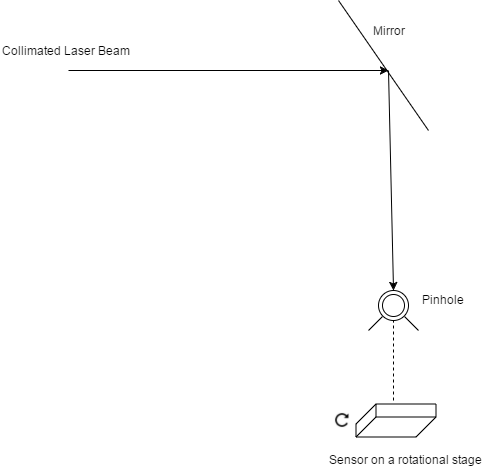
\includegraphics[scale=0.50]{pics/acceptanceCone.png}
\caption{Experimental Setup for detection of acceptance cone}
\label{fig:exp_acc}
\end{figure}

\begin{figure}[ht]
    \centering
    \begin{subfigure}{0.5\textwidth}
    \centering
        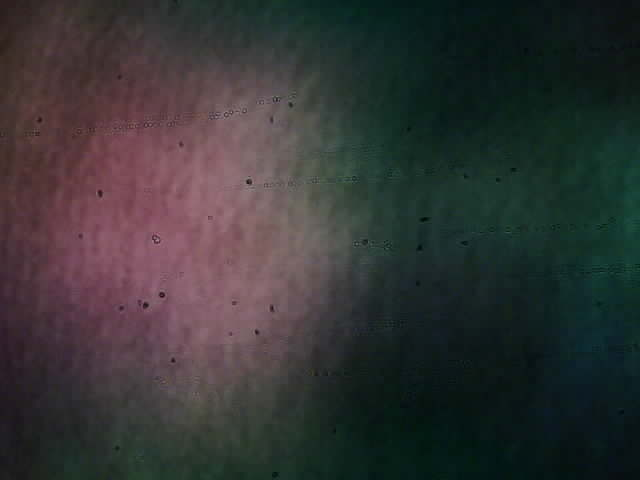
\includegraphics[width=0.5\linewidth]{pics/withoutPinhole.jpg}
        \caption{Image without pinhole}
        \label{fig:nopinhole}
    \end{subfigure}%
    \begin{subfigure}{0.5\textwidth}
    \centering
        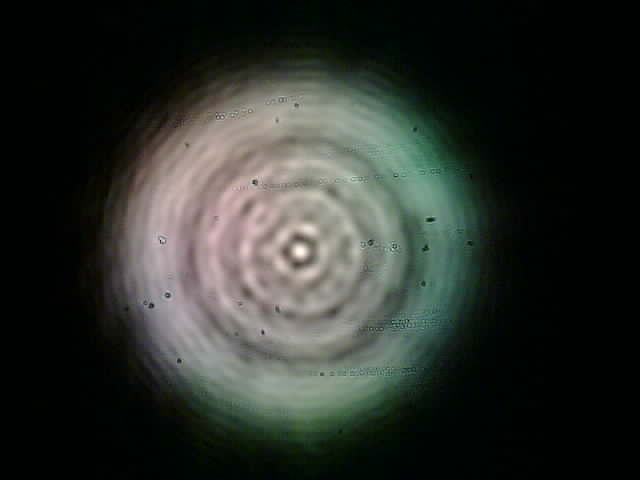
\includegraphics[width=0.5\linewidth]{pics/withPinhole.jpg}
        \caption{Image with pinhole}
        \label{fig:pinhole}
    \end{subfigure}
    \caption{Images of a laser beam caught with and without pinhole}
    \label{fig:pinholeDiff}
    \end{figure}
The pinhole cannot be used to measure the acceptance cone of the sensor because the waveform from the pinhole is a linear combination of different plane waves from different angles. Hence, this measurement was done without a pinhole. In order to measure the acceptance cone of the sensor, it is necessary to identify a portion of the image that can be taken as a reference to plot the variation in the signal measurement. It was assumed that the maximum point in the image can be taken as the signal. Since there was too much variation in the intensities measured, it was decided that we would average the 10 images in each angular position to reduce the signal noise. The maximum value in the image was taken and normalized and the measurements were repeated from -45$\degree$ to +45$\degree$ for 10 sets. The data from the red channel is analyzed. The exposure value was chosen such that the output does not saturate(does not reach 255) for any value in the image(See Figure \ref{fig:exp_acc_exp}). The maximum value in the image versus the angle is plotted. The ideal exposure value would be the one in which the signal does not saturate and there is still some room for additional signals. This is also indicated in Figure \ref{fig:exp_acc_exp}.
\begin{figure}[ht]
\centering
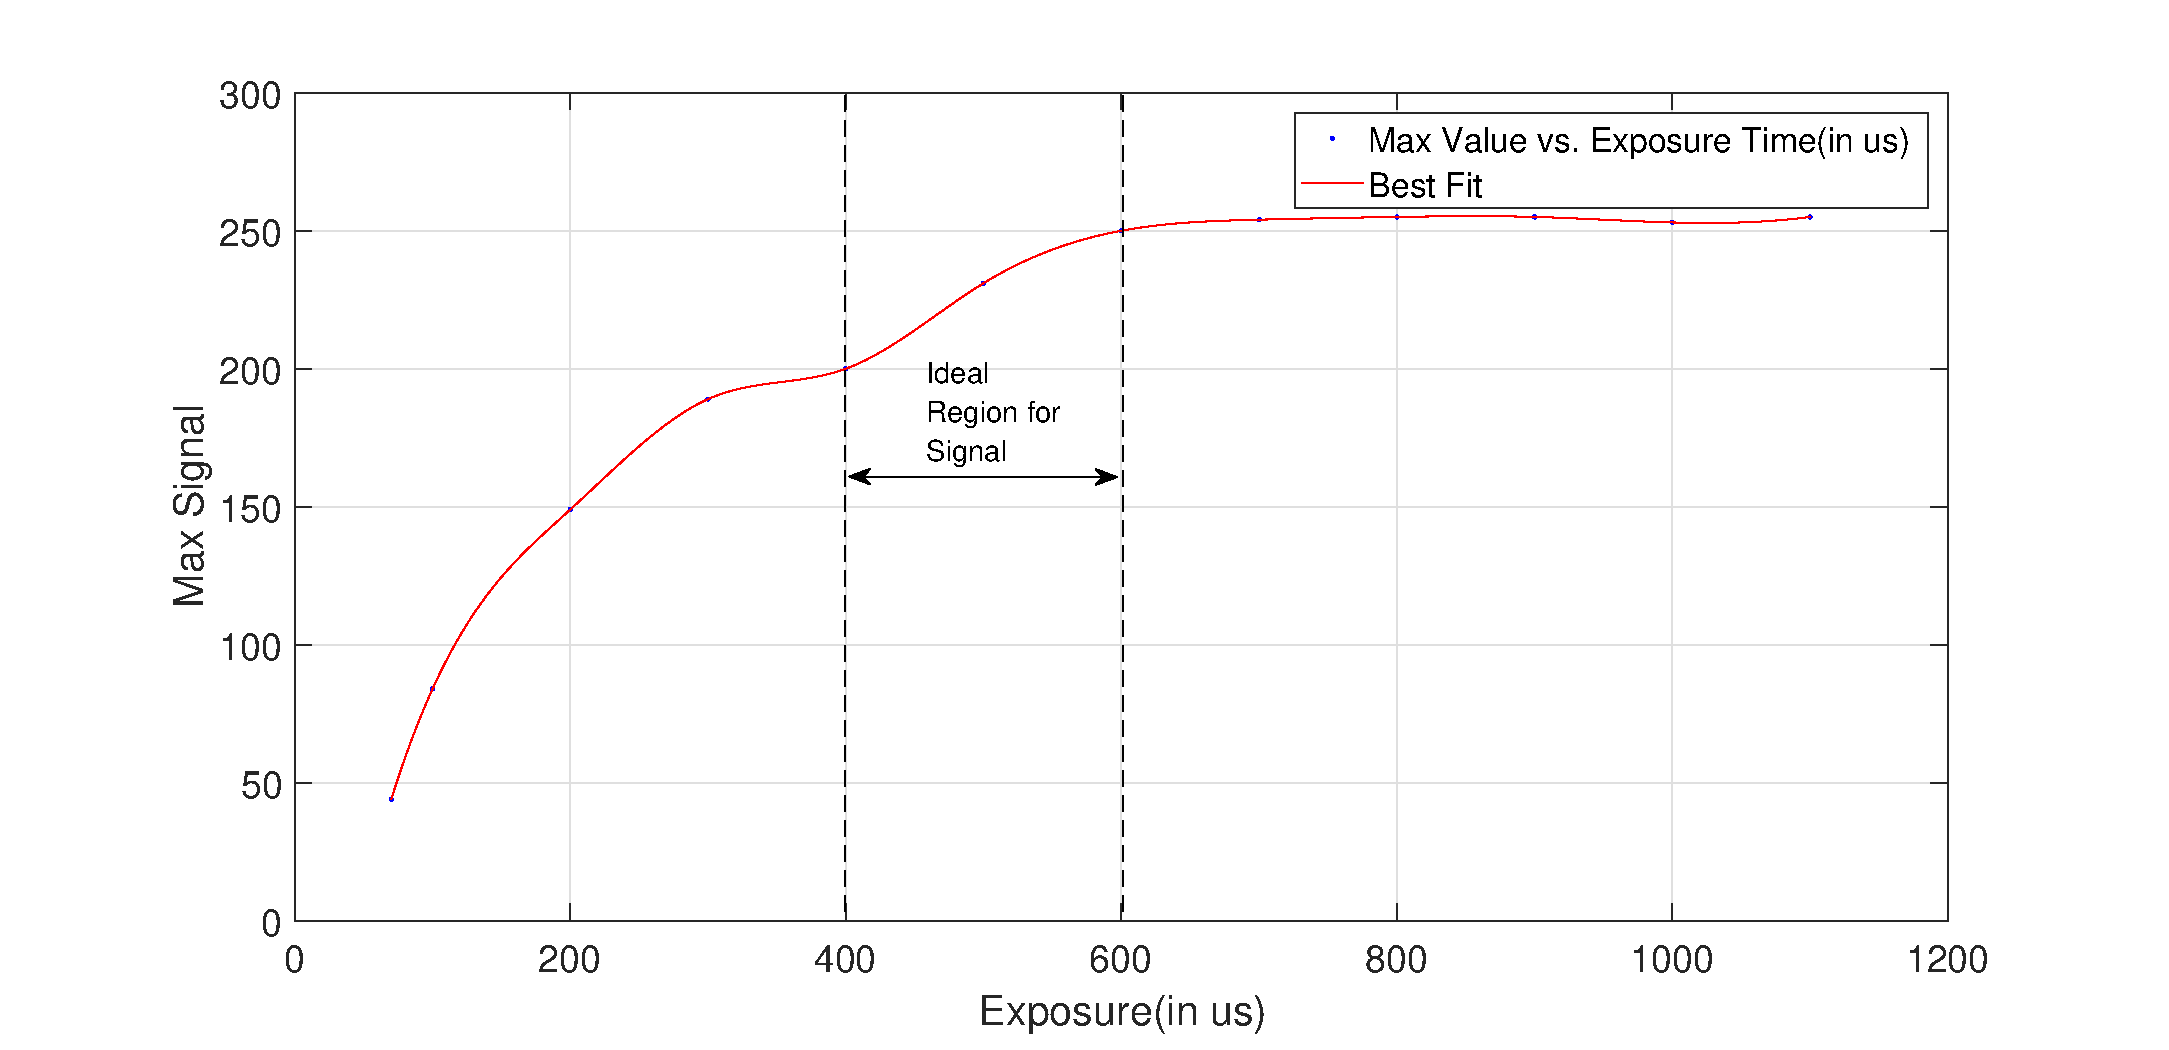
\includegraphics[width = \textwidth]{pics/ExposureTests}
\caption{Response for different Exposure values in microseconds}
\label{fig:exp_acc_exp}
\end{figure}

The obtained response curve for red channel is shown in Figure \ref{fig:exp_acc_red_1}. The normalized signal values are plotted with the standard deviation obtained for each angle are indicated with the use of an error bar. The best obtained curve fit is also plotted.
 \begin{figure}[ht]
\centering
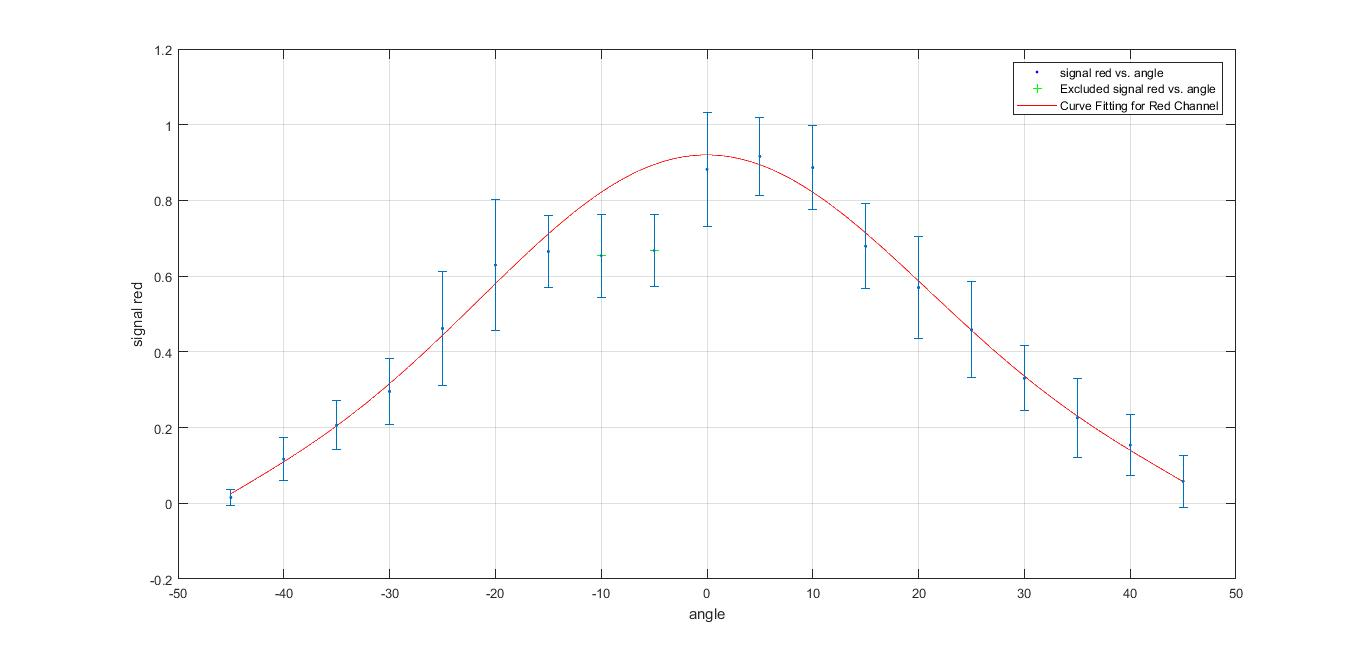
\includegraphics[width = \textwidth]{pics/RedChannel}
\caption{Response for Red Channel in Initial Experiment}
\label{fig:exp_acc_red_1}
\end{figure}

The initial observations from the results obtained are:
\begin{itemize}
\item There seems to be a very large standard deviation for each angle.
\item There seems to very sharp outliers at -5$\degree$ and -10$\degree$ which is a highly unexpected behavior.
\end{itemize}
These two observations point to experimental error. The error in the experimental results could be due to the following reasons:
\begin{itemize}
\item \textbf{Error introduced due to the translation of the rotational stage :} In order to make sure that the beam always hits the stage is translated if the beam does not hit due to the translation of the sensor away from the beam. This introduces an additional angular error which is not taken into account in the initial experiment. So, the stage was calibrated using the pinhole. If the sensor is exactly at the center of rotation of the rotational stage, the laser beam must always hit the same position of the sensor no matter what the rotational angle may be. The position of the sensor on the rotational stage was calibrated such that the signal(image with pinhole) obtained always remained at the center of the sensor. 

\item \textbf{Improper Reference Signal from Image :} At times, it was observed that the maximum point in the image occurs at different and unexpected points that are outside the beam. This also leads to different parts of the signal being measured each time. The outliers in the results could also mean that. An example average image in which the maximum is obtained at the end of the beam is shown in Figure \ref{fig:exp_acc_improper}. The point from where the signal is obtained is marked using a yellow star in the Figure \ref{fig:exp_acc_improper}.
\begin{figure}[ht]
\centering
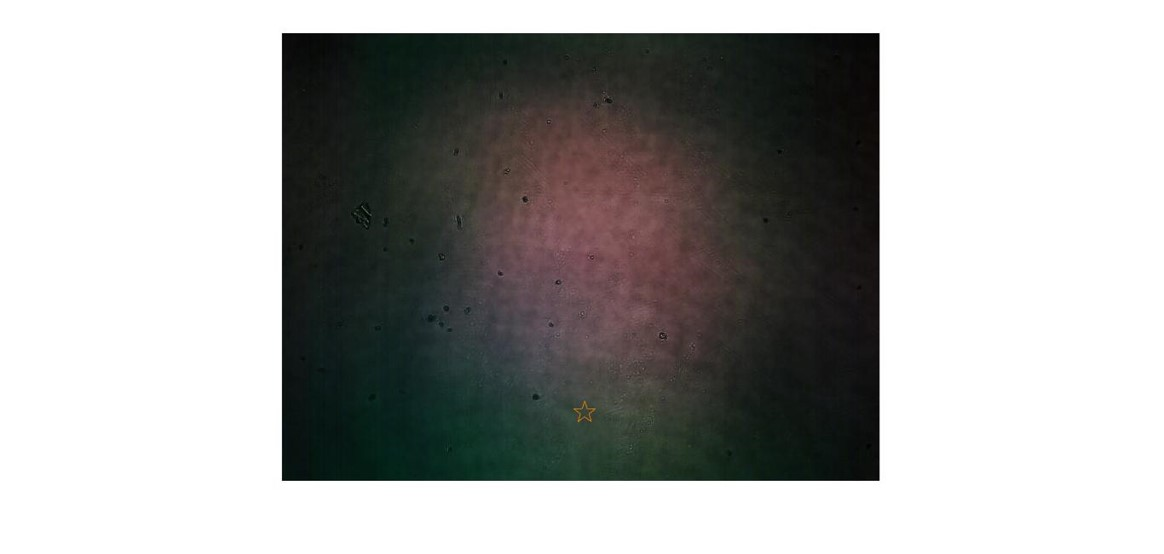
\includegraphics[width = 0.75\textwidth]{pics/ImproperDetection}
\caption{Improper Reference Point for Signal}
\label{fig:exp_acc_improper}
\end{figure}
\item \textbf{Large Variation in the intensity of output image :} It was noticed that there was a huge variation in intensity for subsequent measurements at the very subsequent instants. This variation in the output is the cause of the large standard deviation in the result. Initially, I thought that this could be due to a relatively low exposure time(as lower exposure could lead to more output noise) or due to the variation of intensity of laser beam. Increasing the exposure time did give lower variations but the problem was traced to the automatic gain control(AGC) in the OV2640 image sensor. The amplifier gain of each pixel was adjusted automatically and this led to different intensities in subsequent readings. After this feature was turned off by modifying the driver software using I2C, it seemed that the variation in the output was no longer there.

\item \textbf{Unexpected Colors in the output image :} An unexpected feature in the image is seen in each measurement. The unexpected feature is the presence of green and blue colors of the laser beam. Since the laser beam is red with an almost constant wavelength in the red visible light region, the output of green is unexpected. This was very strange and upon studying the sensor, it seemed that the sensor had an automatic white balance(AWB) feature of OV2640. This white balance feature assumes a ``gray" world(wherein the average of all colors in the world is gray)\cite{OV2640SoftwareApp} which is not true in our case. The difference in the output is with and without AWB is shown in Figure \ref{fig:AWB}. Even after this adjustment, there seems to be a slight tinge of green at negative angles where the beam seems to ``dim" out. Even after trying out a variety of different settings this green could not be eliminated and could be due to Black Level Calibration in the sensor. The function of Black Level Calibration (BLC) is to produce accurate color in the dark area of the picture. There is no mention of how to turn off this feature in the datasheet or the application notes of this sensor. The vendor of the camera did not provide any information on how to turn off this feature. Hence, it was assumed that the sensor does not make any modifications to the red channel in angles where the signal ``dims" out.
\begin{figure}[ht]
    \begin{subfigure}{0.5\textwidth}
    \centering
        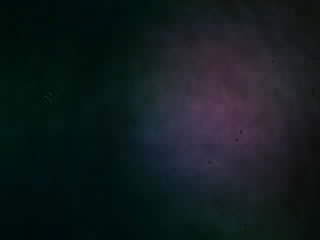
\includegraphics[width=0.5\linewidth]{pics/awb.jpg}
        \caption{Image with AWB}
    \end{subfigure}%
    \begin{subfigure}{0.5\textwidth}
    \centering
        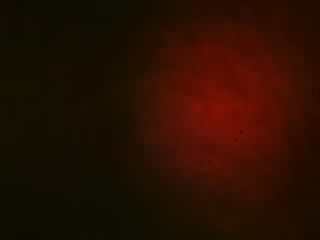
\includegraphics[width=0.5\linewidth]{pics/withoutawb.jpg}
        \caption{Image without AWB}
    \end{subfigure}
    \caption{Images of a laser beam caught with and without pinhole}
    \label{fig:AWB}
    \end{figure}
\end{itemize}
\subsection{Improved experiment}
As mentioned in the previous experiment, the stage was calibrated such that the sensor remains at the center of rotation of the rotational stage. The reference signal was chosen such that the same point of the beam is always measured. In order to make sure that the same point of the beam is measured with and without pinhole, the coordinate of the central diffraction pattern is stored for different angular positions for -45$\degree$ to +45$\degree$ and the reference signal is taken from this point. In order to detect the central region in the output, a function called \texttt{imfindcircles} is used\cite{imfindcircles}. This function finds circles in an image using circular Hough transform. The readings for a specific angle are averaged and a logarithmic function is applied which is then passed to the \texttt{imfindcircles} function to detect the brightest possible circle with a radius of 3 pixels(This value was tuned such that the central portion is detected with 100 percent accuracy). The detection process using this method provided 100 percent accuracy for detection of the center of the central fringe pattern coordinate. This is illustrated in Figure \ref{fig:center_calib}. The Automatic gain controls and Automatic White balance features of the CMOS sensors were turned off by using suitable register settings mentioned in \cite{OV2640DS}. The Arduino was programmed to set the register values using I2C. The exposure was set at 500$\mu$s based on the exposure graph(See Figure \ref{fig:exp_acc_exp}).
\begin{figure}[!h]
\centering
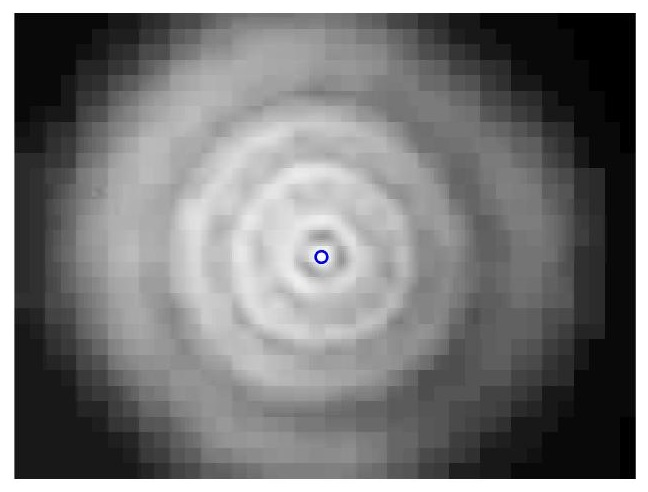
\includegraphics[scale=0.300]{pics/CentralRegionTracking.jpg}
\caption{Coordinate Detection for central region signal detection}
\label{fig:center_calib}
\end{figure}

In the first step of the experiment, the rotational stage is rotated from -45$\degree$ to +45$\degree$ with pinhole and the coordinates of the central diffraction pattern is stored in a variable. In the second step of the experiment, the pinhole is removed and the signal is taken for different angles from the center coordinates measured using the diffraction pattern. This will ensure that we measure the same part of the beam every time we take a signal for measurement. After this, the signal is taken with a different offset(from the central diffraction pattern) in the X-direction to make sure that all the pixels behave in the same manner. The graphs for 100 different pixel positions in X-direction from the central position is shown in Figure \ref{fig:offset_calib}. From this graph, it can be seen that all the pixels in the same line exhibit the same behavior with a slight shift in angular position peak. In figure \ref{fig:offset_calibY}, the response for different pixels in the Y-direction is shown. It can be seen that there is a wider variation in the curve peak position. It can also be seen that all the pixels follow the same pattern with a slight shift in the peaks.
\begin{figure}[!h]
\centering
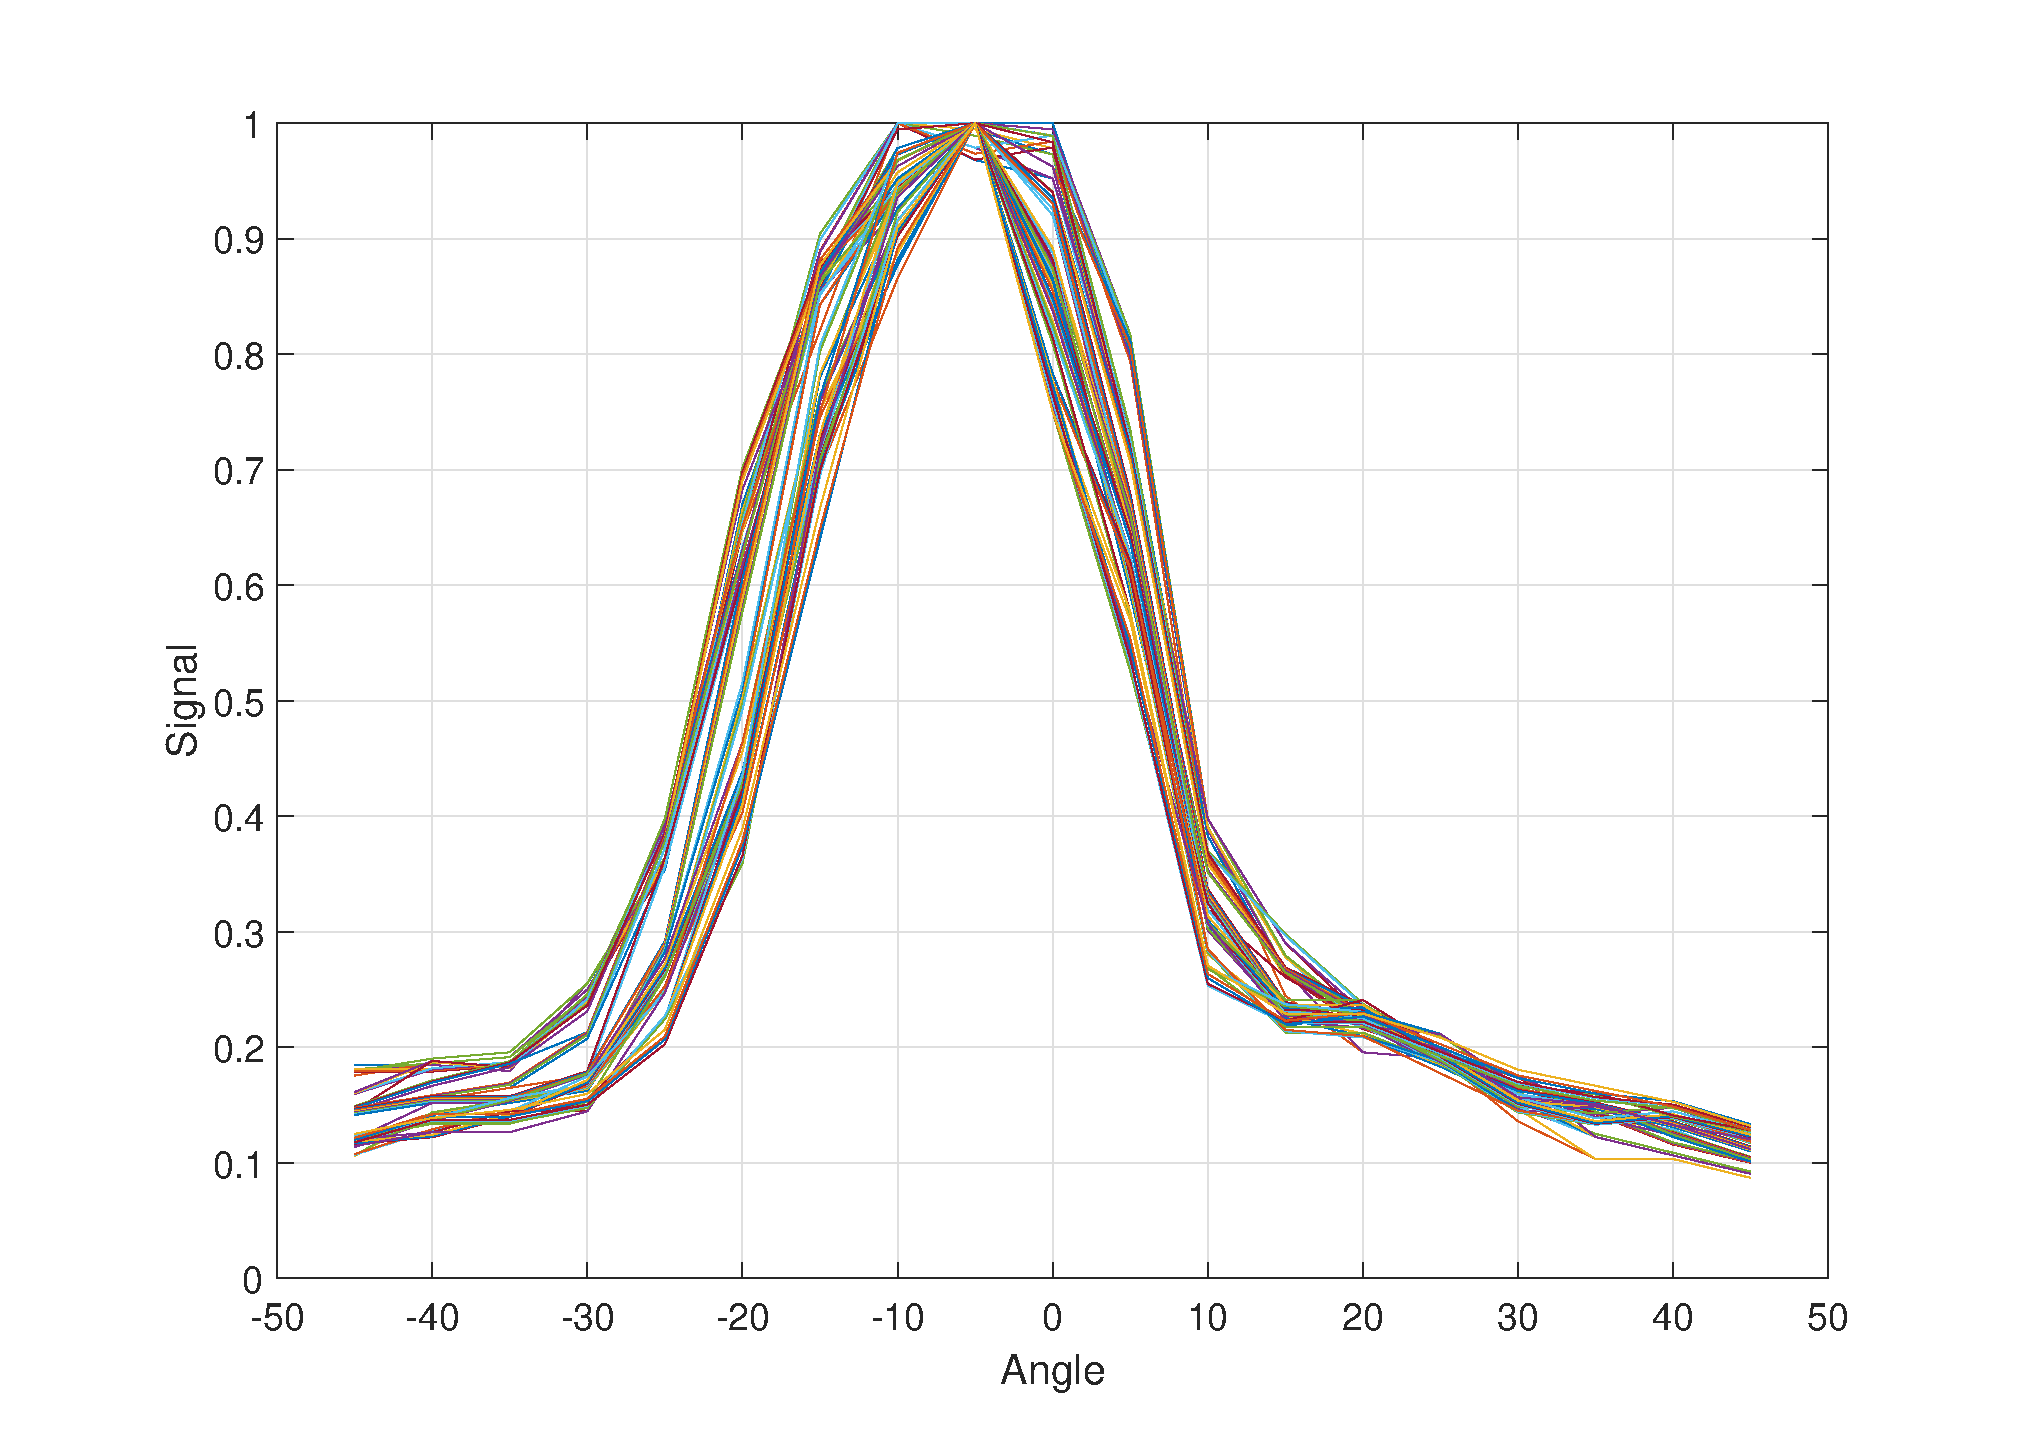
\includegraphics[width = 0.90\textwidth]{pics/ResponseXOffset}
\caption{Response for 100 different offset pixel positions from central diffraction pattern in X-direction}
\label{fig:offset_calib}
\end{figure}

\begin{figure}[!h]
\centering
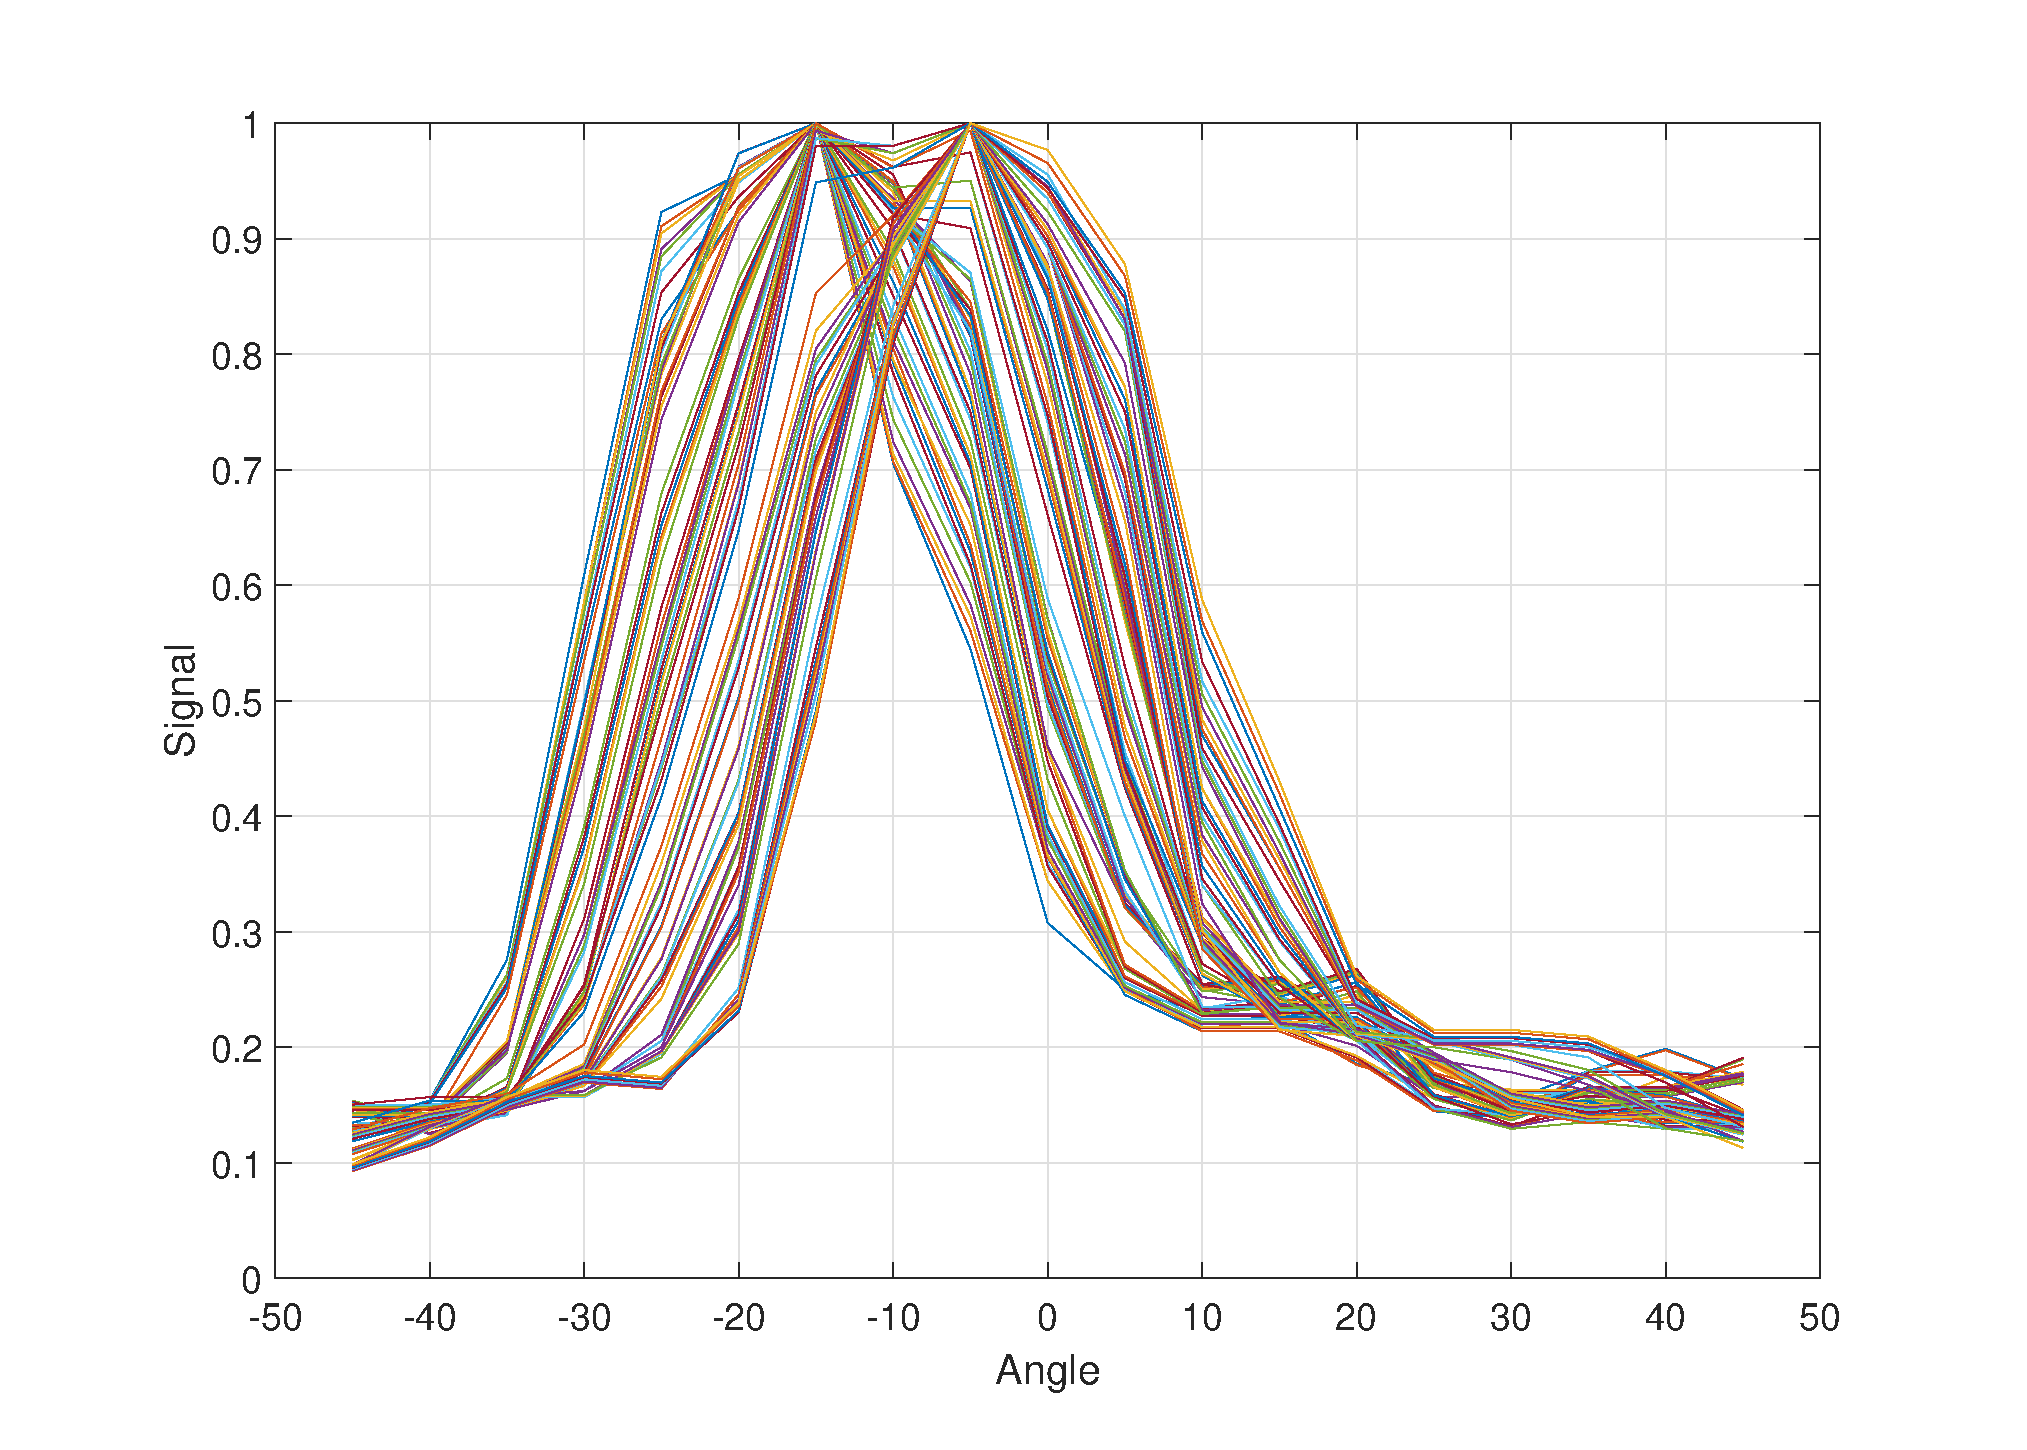
\includegraphics[width = 0.90\textwidth]{pics/ResponseYOffset}
\caption{Response for 100 different offset pixel positions from central diffraction pattern in Y-direction}
\label{fig:offset_calibY}
\end{figure}

The peak positions for different pixel offset positions in the X and Y direction is shown in \ref{fig:peak_pixel_pos}. It can be seen that pixels in the same neighborhood have the same peak angular positions. The shift in peak is seen as we move across the detector.  The peak angular position for different pixel positions is shown in Figure \ref{fig:peak_pixel_pos}.
This can be attributed to the non-uniformity in the laser beam that is used for measuring the response of the pixels.
\begin{figure}[!h]
\centering
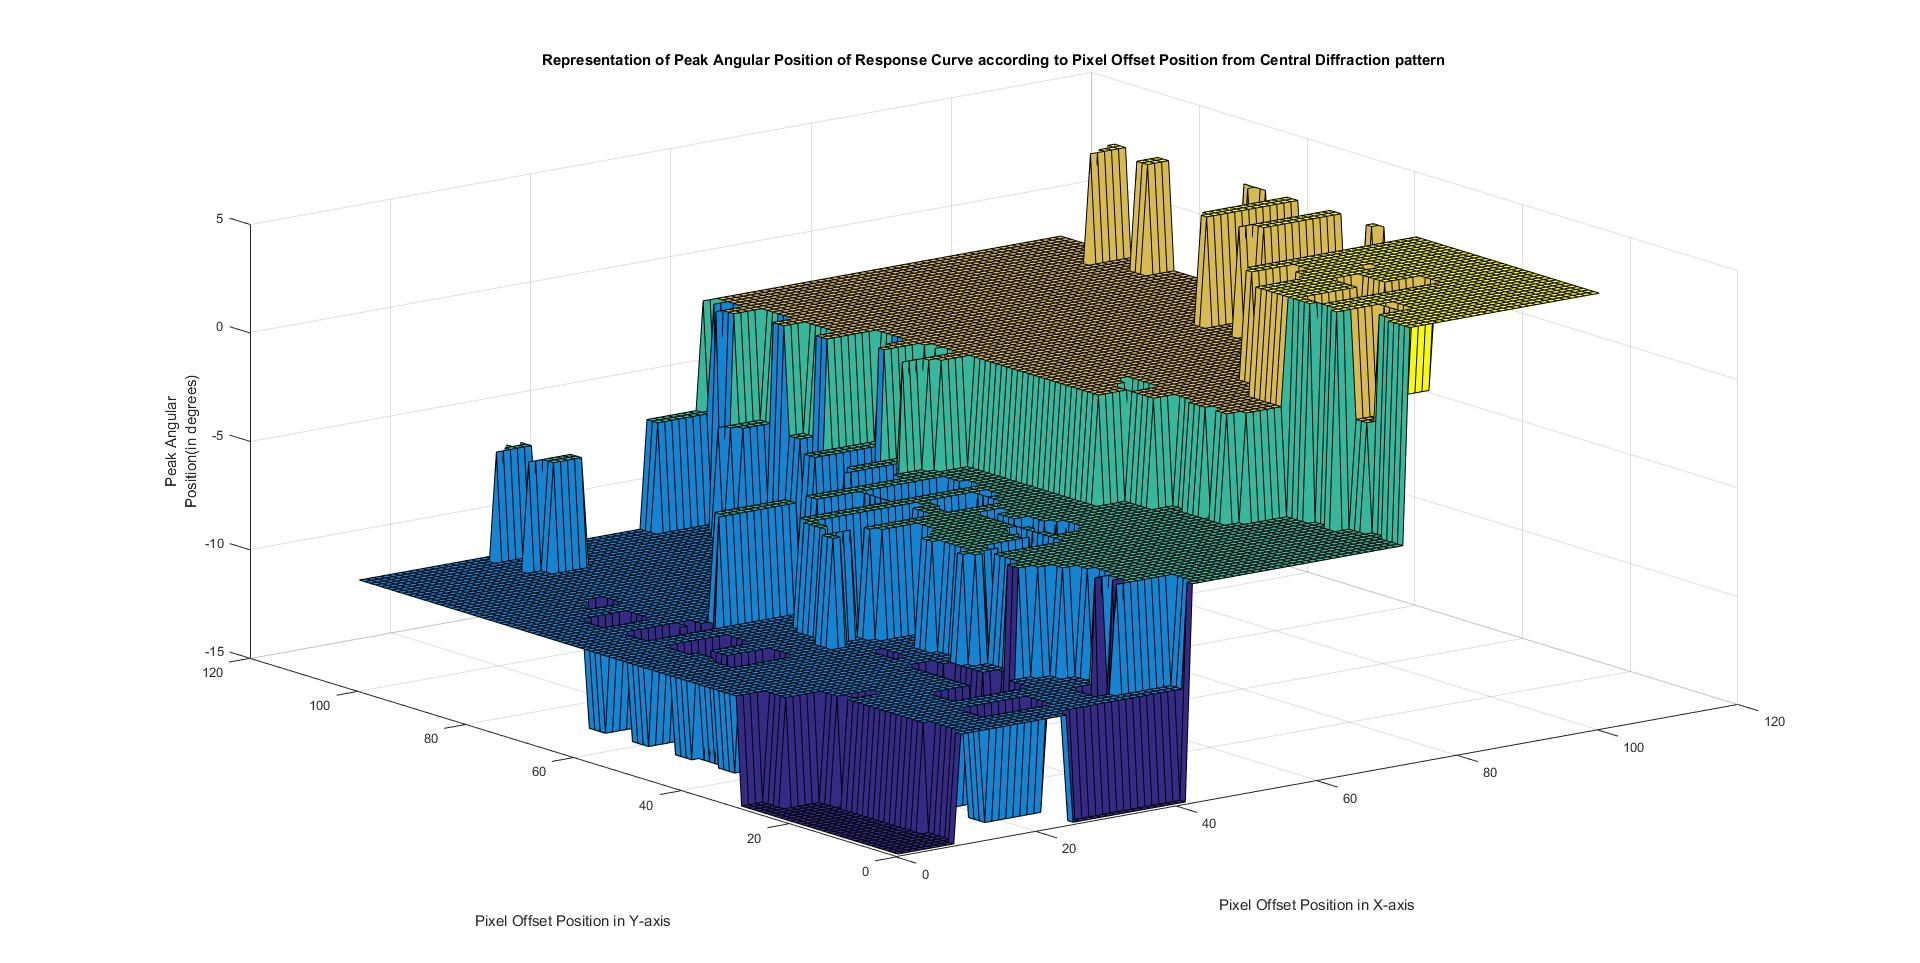
\includegraphics[width = \textwidth]{pics/MeshPlotAngularPeak}
\caption{Peak Angular Positions for different Pixels}
\label{fig:peak_pixel_pos}
\end{figure}

The experiment is repeated for 10 times and the response is plotted only for the red channel as we have only red frequency light hitting the sensor beam. The final result after solving the problems mentioned in the previous section is shown in Figure \ref{fig:acceptance_final}.
\begin{figure}[!h]
\centering
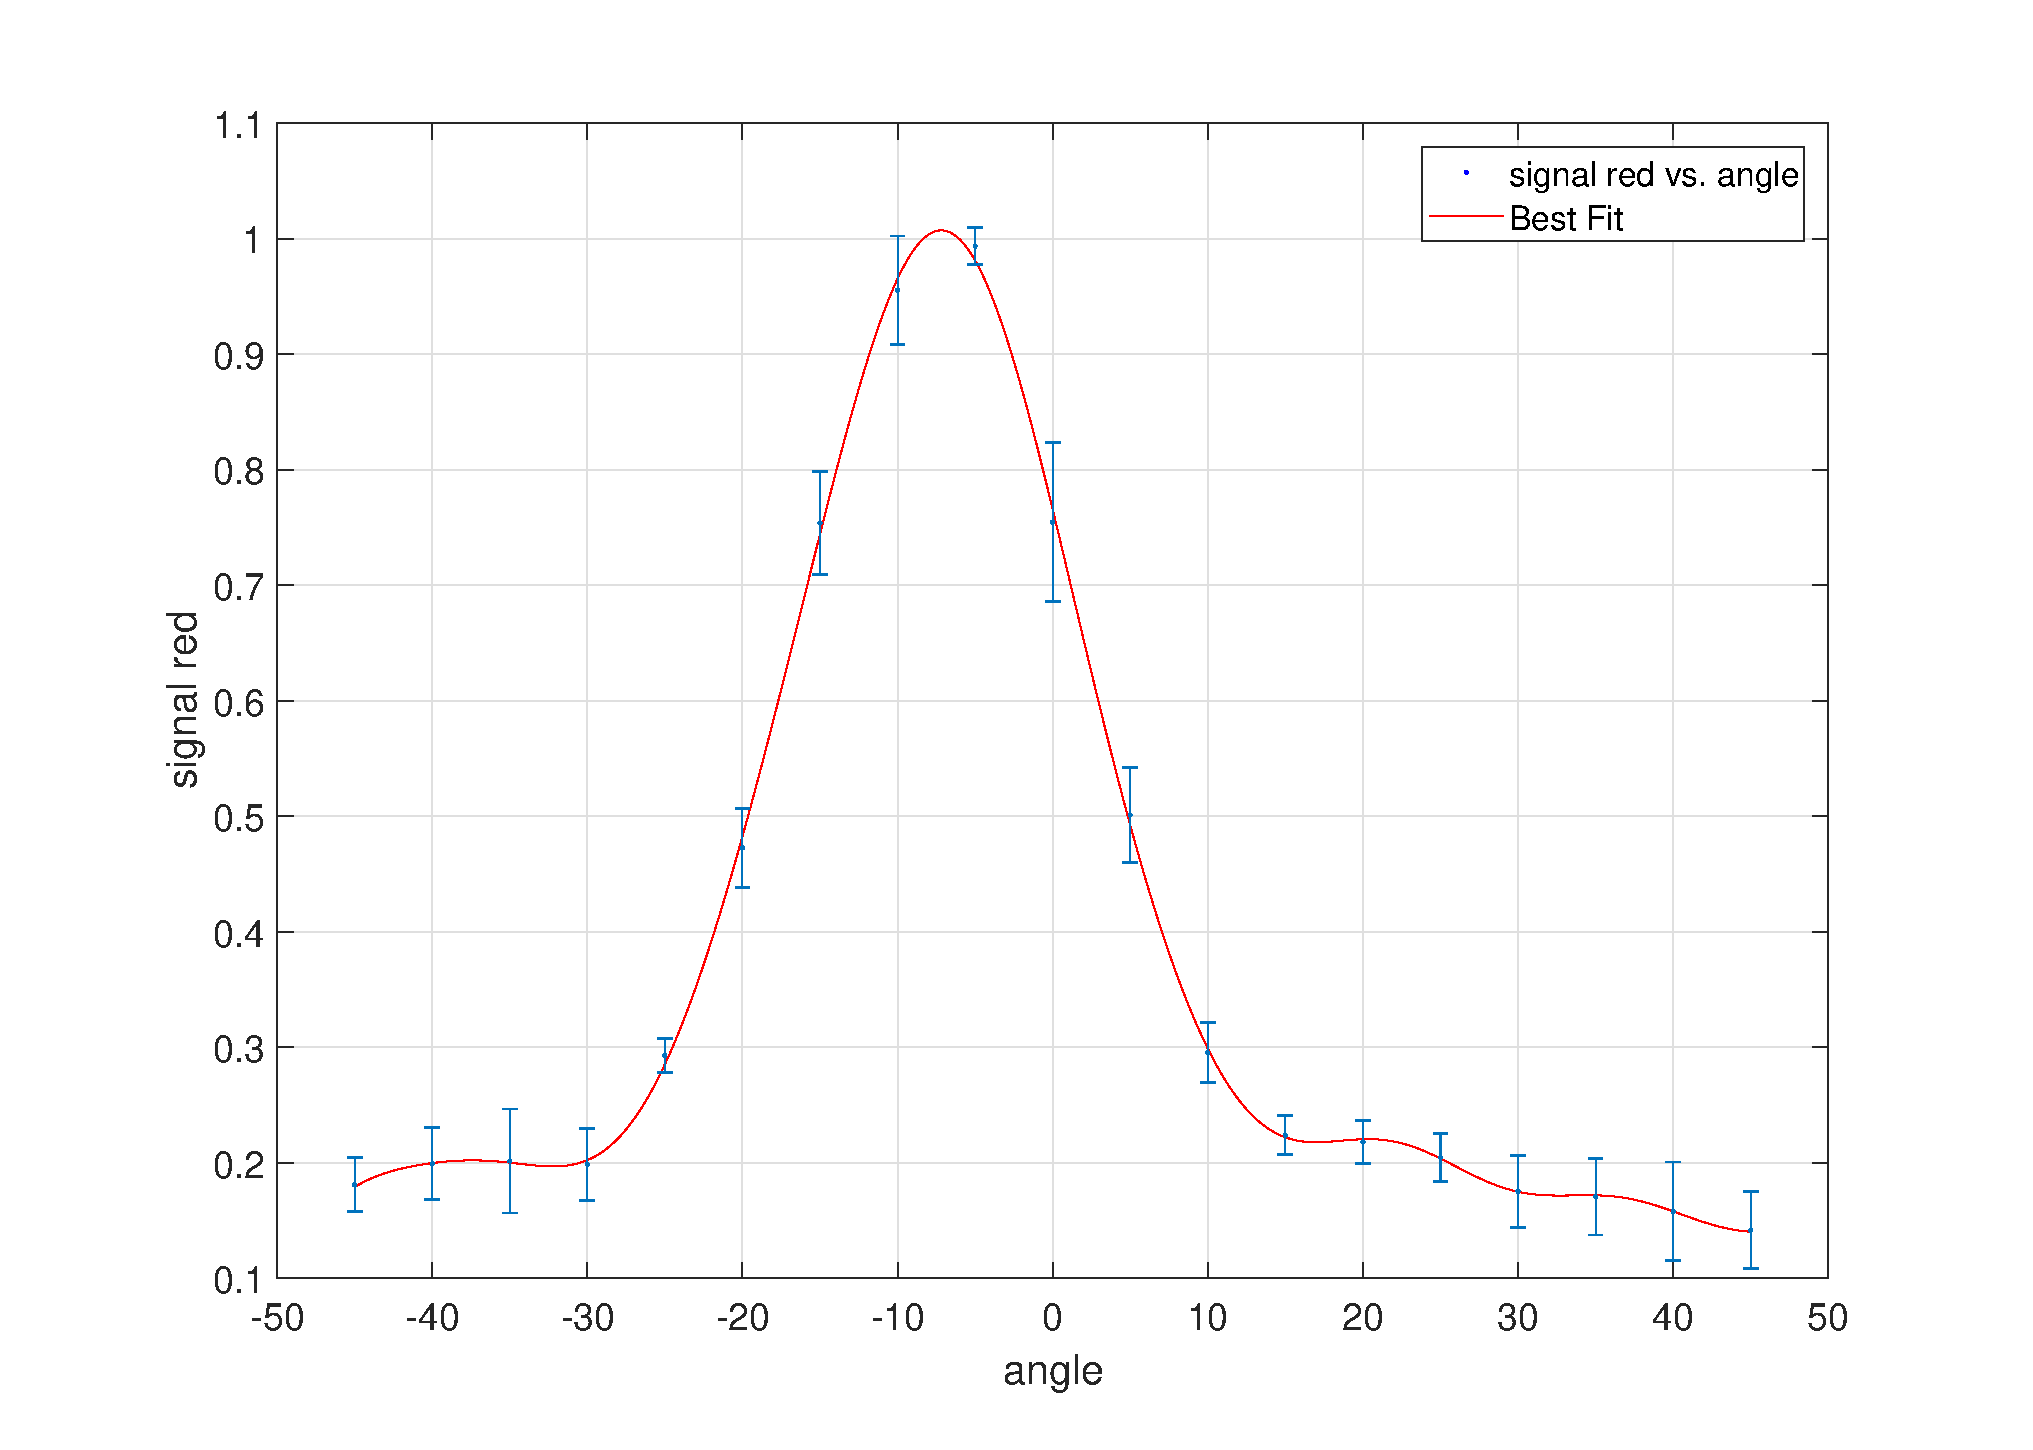
\includegraphics[width = \textwidth]{pics/FinalCRAExp}
\caption{Finalized Red Channel Response for Different Data Sets}
\label{fig:acceptance_final}
\end{figure}
There is less overlap in the subsequent angles and no points are excluded in the curve fitting process. The maximum standard deviation was reduced from 16 percent for the angular position -20(See Figure \ref{fig:exp_acc_red_1}) to 6 percent for angular position 0(See Figure \ref{fig:acceptance_final}). The peak of the curve is shifted towards -5$\degree$ because the maximum position of the laser beam occurs at -5$\degree$ position of the rotational beam. The graph data needs to be incorporated into the simulation to see the effect of the acceptance cone of the sensor on the image reconstruction. This will be discussed in the subsequent section.
\section{Adding to Simulation}
The curve data that was obtained in the previous experiment was incorporated into the previously obtained simulation results. In order to incorporate the data, we need to generate a 2-dimensional matrix that would simulate the behavior of the acceptance cone effect on the reconstruction. Since the behavior will be exhibited in both the horizontal and vertical directions, the 1-D curve was converted into 2-D by multiplying itself with its transpose. This would generate a circular symmetric matrix that would generate the effect of the acceptance cone in both the horizontal and vertical directions. This is shown in Figure \ref{fig:curve_sim}. We increase the effective interest area from $512 \times 512$ to $1024 \times 1024$ to visually see the number of pixels lost due to the acceptance angle effects. The mask size is changed accordingly to suit the image size.   
\begin{figure}[!h]
\centering
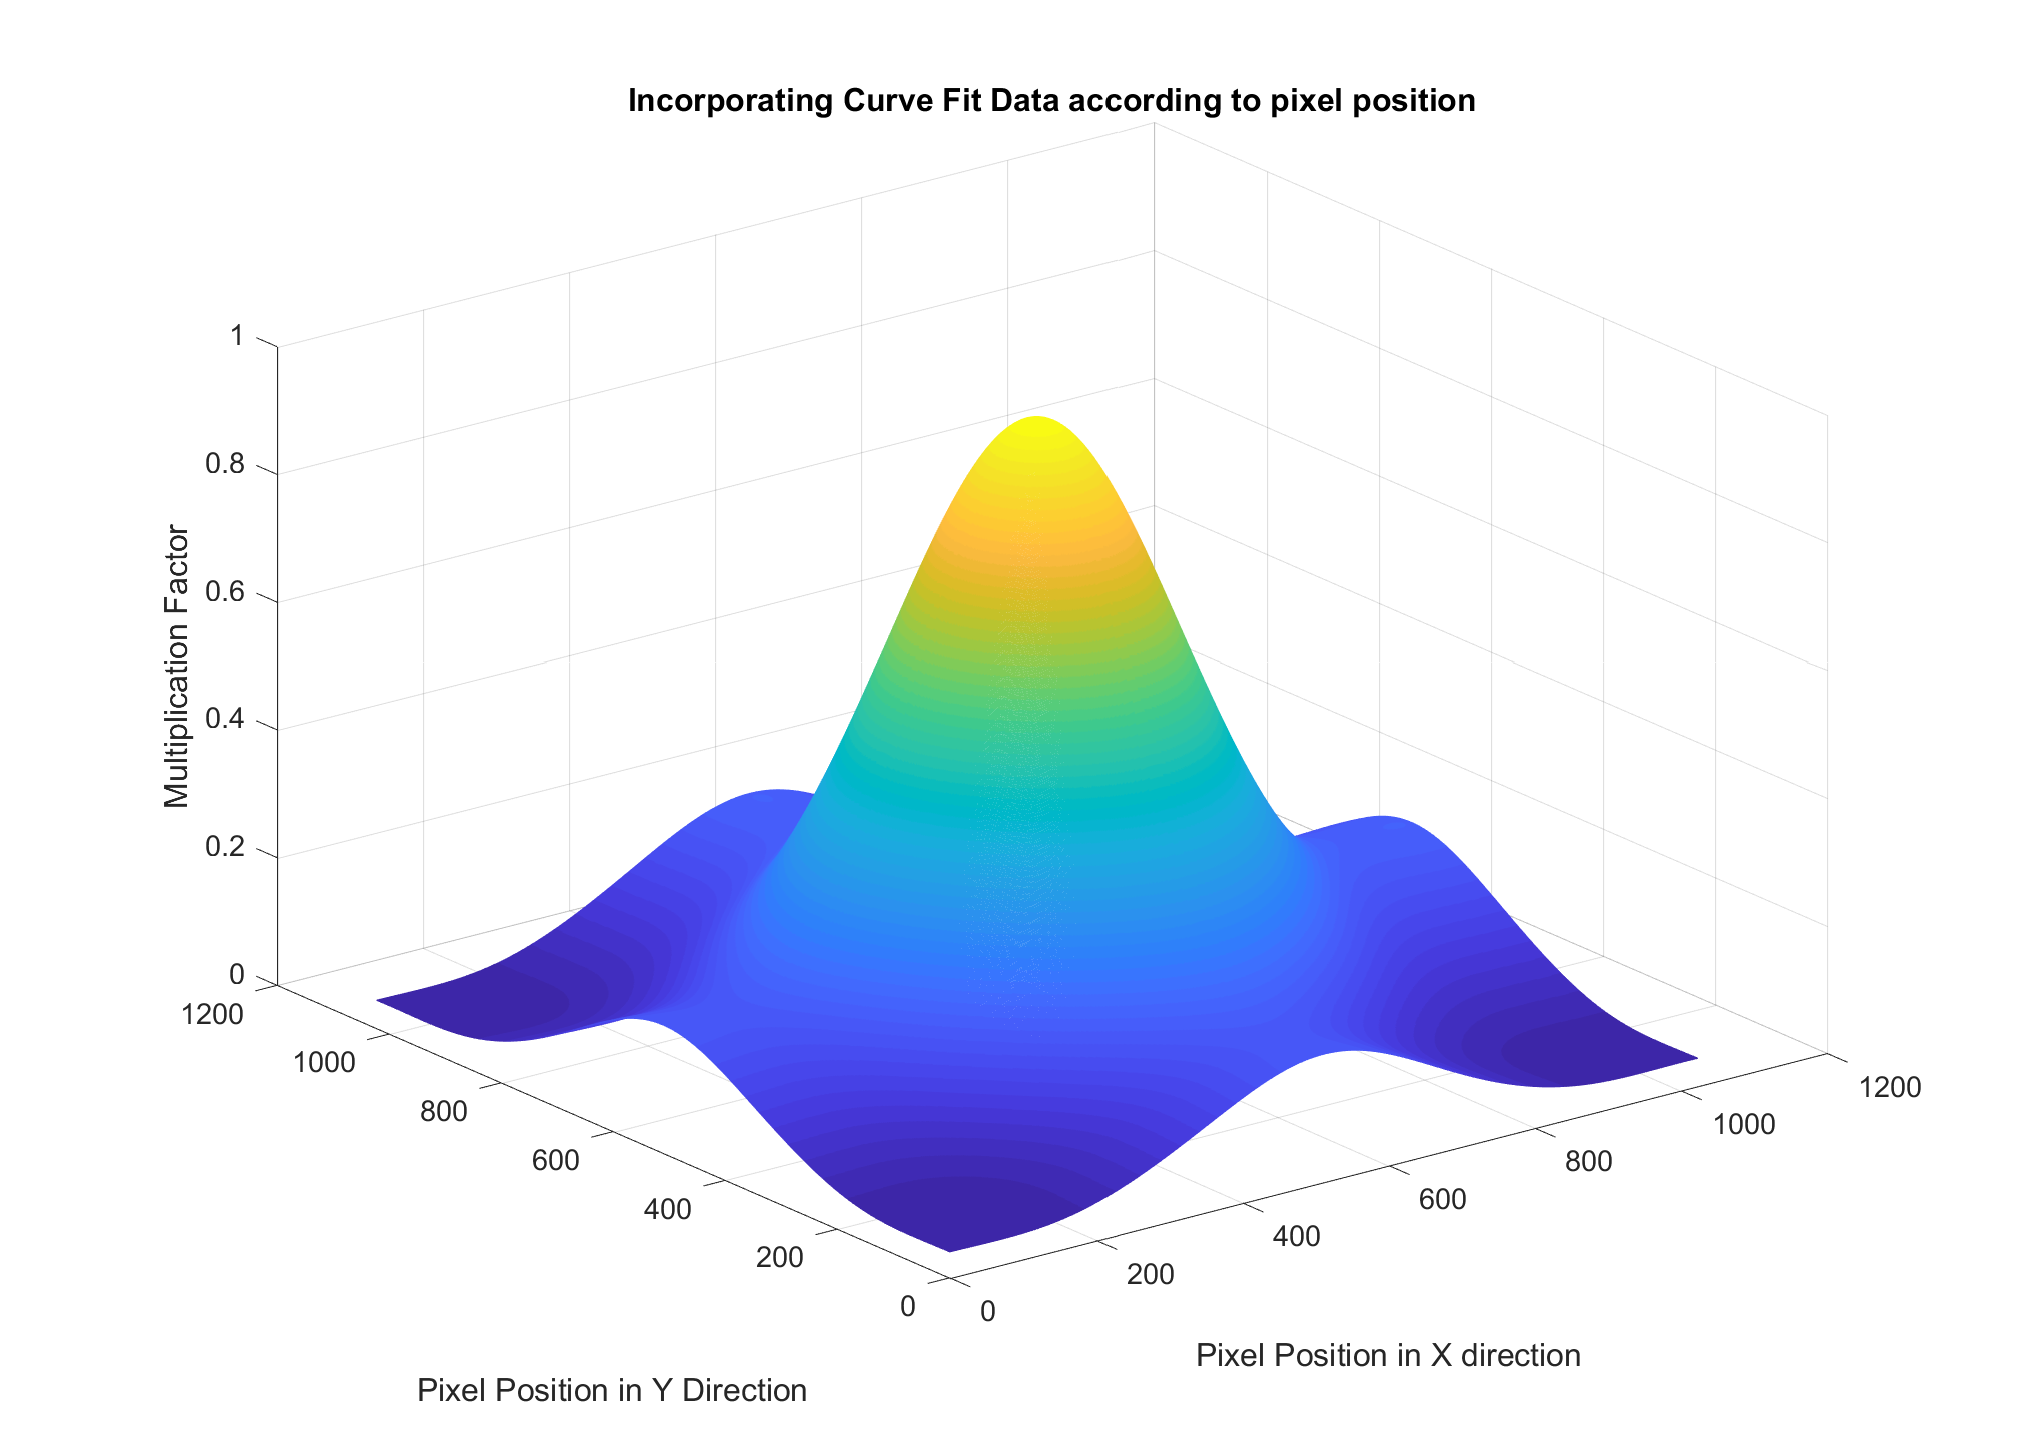
\includegraphics[width = \linewidth]{pics/AcceptanceConeCurveFit}
\caption{Fitted Curve Data into simulation}
\label{fig:curve_sim}
\end{figure}
This matrix is multiplied with the original image to simulate the effect of angle acceptance on the image reconstruction. This was tried with the simulation results that simulate the effects of diffraction to simulate as close to a real world. The source image, the reconstruction only with diffraction effects and the reconstruction with diffraction and acceptance cone is shown in Figure \ref{fig:rec_acc}. It can be seen that reconstruction with diffraction effects lead to a slight loss of detail. Once we incorporate the effects of acceptance cone into the simulation, it can be seen that only a portion of the original image can be reconstructed which is indicated by the square box in Figure \ref{fig:rec_acc}. 
This would be the actual field of view in the real world.  In order to find the angular field of view, the positions of the square box must be correlated with the fitted matrix curve discussed. On doing this, it can be found that the area in the rectangular box corresponds to an angle of -21.7$\degree$ to +21.7$\degree$. The angular field of view in absolute terms will be 43.4$\degree$ in the horizontal direction. The horizontal field of view and the vertical field of view can be considered to be equal since the pixel size of the CMOS sensor(OV2640) is the same in both directions.

 \begin{figure}[!h]
\centering
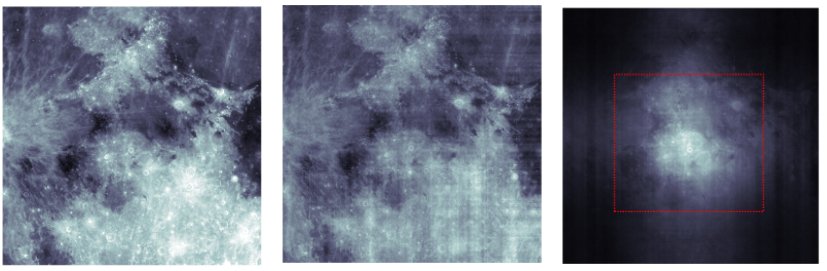
\includegraphics[width = \linewidth]{pics/ReconstructionAcce}
\caption{The image on the left indicates the original object image, the image in the middle indicates the reconstruction with only diffraction effects. The image on the right indicates both diffraction and acceptance angle effects. The red area indicates the effective amount of pixels that can be used. }
\label{fig:rec_acc}
\end{figure}
    

A lens based system would have a larger field of view depending on the lens used. The OV2640 camera module by default comes with a 1.4-inch lens with a field horizontal and vertical acceptance angle of $70\degree \times 63.7\degree$\cite{OV2640Arducam}\cite{lenses}. The lensless system would have a horizontal and vertical acceptance angle of view of $43.4\degree \times 43.4\degree$. This leads to a field of view reduction of 38 percent and 31.8 percent in the horizontal and vertical directions. The effective pixels that can be used by the camera is reduced to 48 percent meaning that only 48 percent of the total number of active pixels can be used for effective imaging. This is the trade-off that we need to face when we reduce the size of the camera by removing the lenses.

\section{Actual Field of View and Spatial Resolution Calculations}
In this section, we will be discussing how we can calculate the field of view of the camera from the experiment and will also perform spatial resolution calculations. This will give us an idea of how the camera will perform when used in an actual space application. The spatial resolution can be calculated using equation \ref{eq:spat_res_2}. 

\begin{equation}
\label{eq:spat_res_2}
d_s = \frac{d_p}{d_t} * d_h
\end{equation}

The calculated spatial resolutions($d_s$) based on mask-sensor distance($d_t$) and the height of the satellite($d_h$) from the earth is shown in Figure \ref{fig:spat-res-graph-1}. It can be seen from the graph that as we increase the mask-sensor distance, we can attain better spatial resolutions that can represent the ground data better. the best spatial resolution is obtained when the mask-sensor distance is the greatest(i.e 10 mm) and when the satellite is as close to the earth(350 kilometers). The best possible spatial resolution can be achieved at a height of 350 kilometers which would be 77 meters per pixel for a mask-sensor distance of 10 mm. A mask-sensor distance of 5 mm would provide 154 meters per pixel at the same height. It can be seen that if we make the camera thicker, we can get better spatial resolutions. The figure \ref{fig:spat-res-graph-1} is calculated for a pixel size of $2.2 \ \mu m \times 2.2 \ \mu m$. The other sensor OV5642 can offer a better spatial resolution as it's pixel size is smaller $1.4 \ \mu m \times 1.4 \ \mu m$. The spatial resolution values will be scaled by the ratio of the pixel sizes. 

\begin{figure}[]
\centering
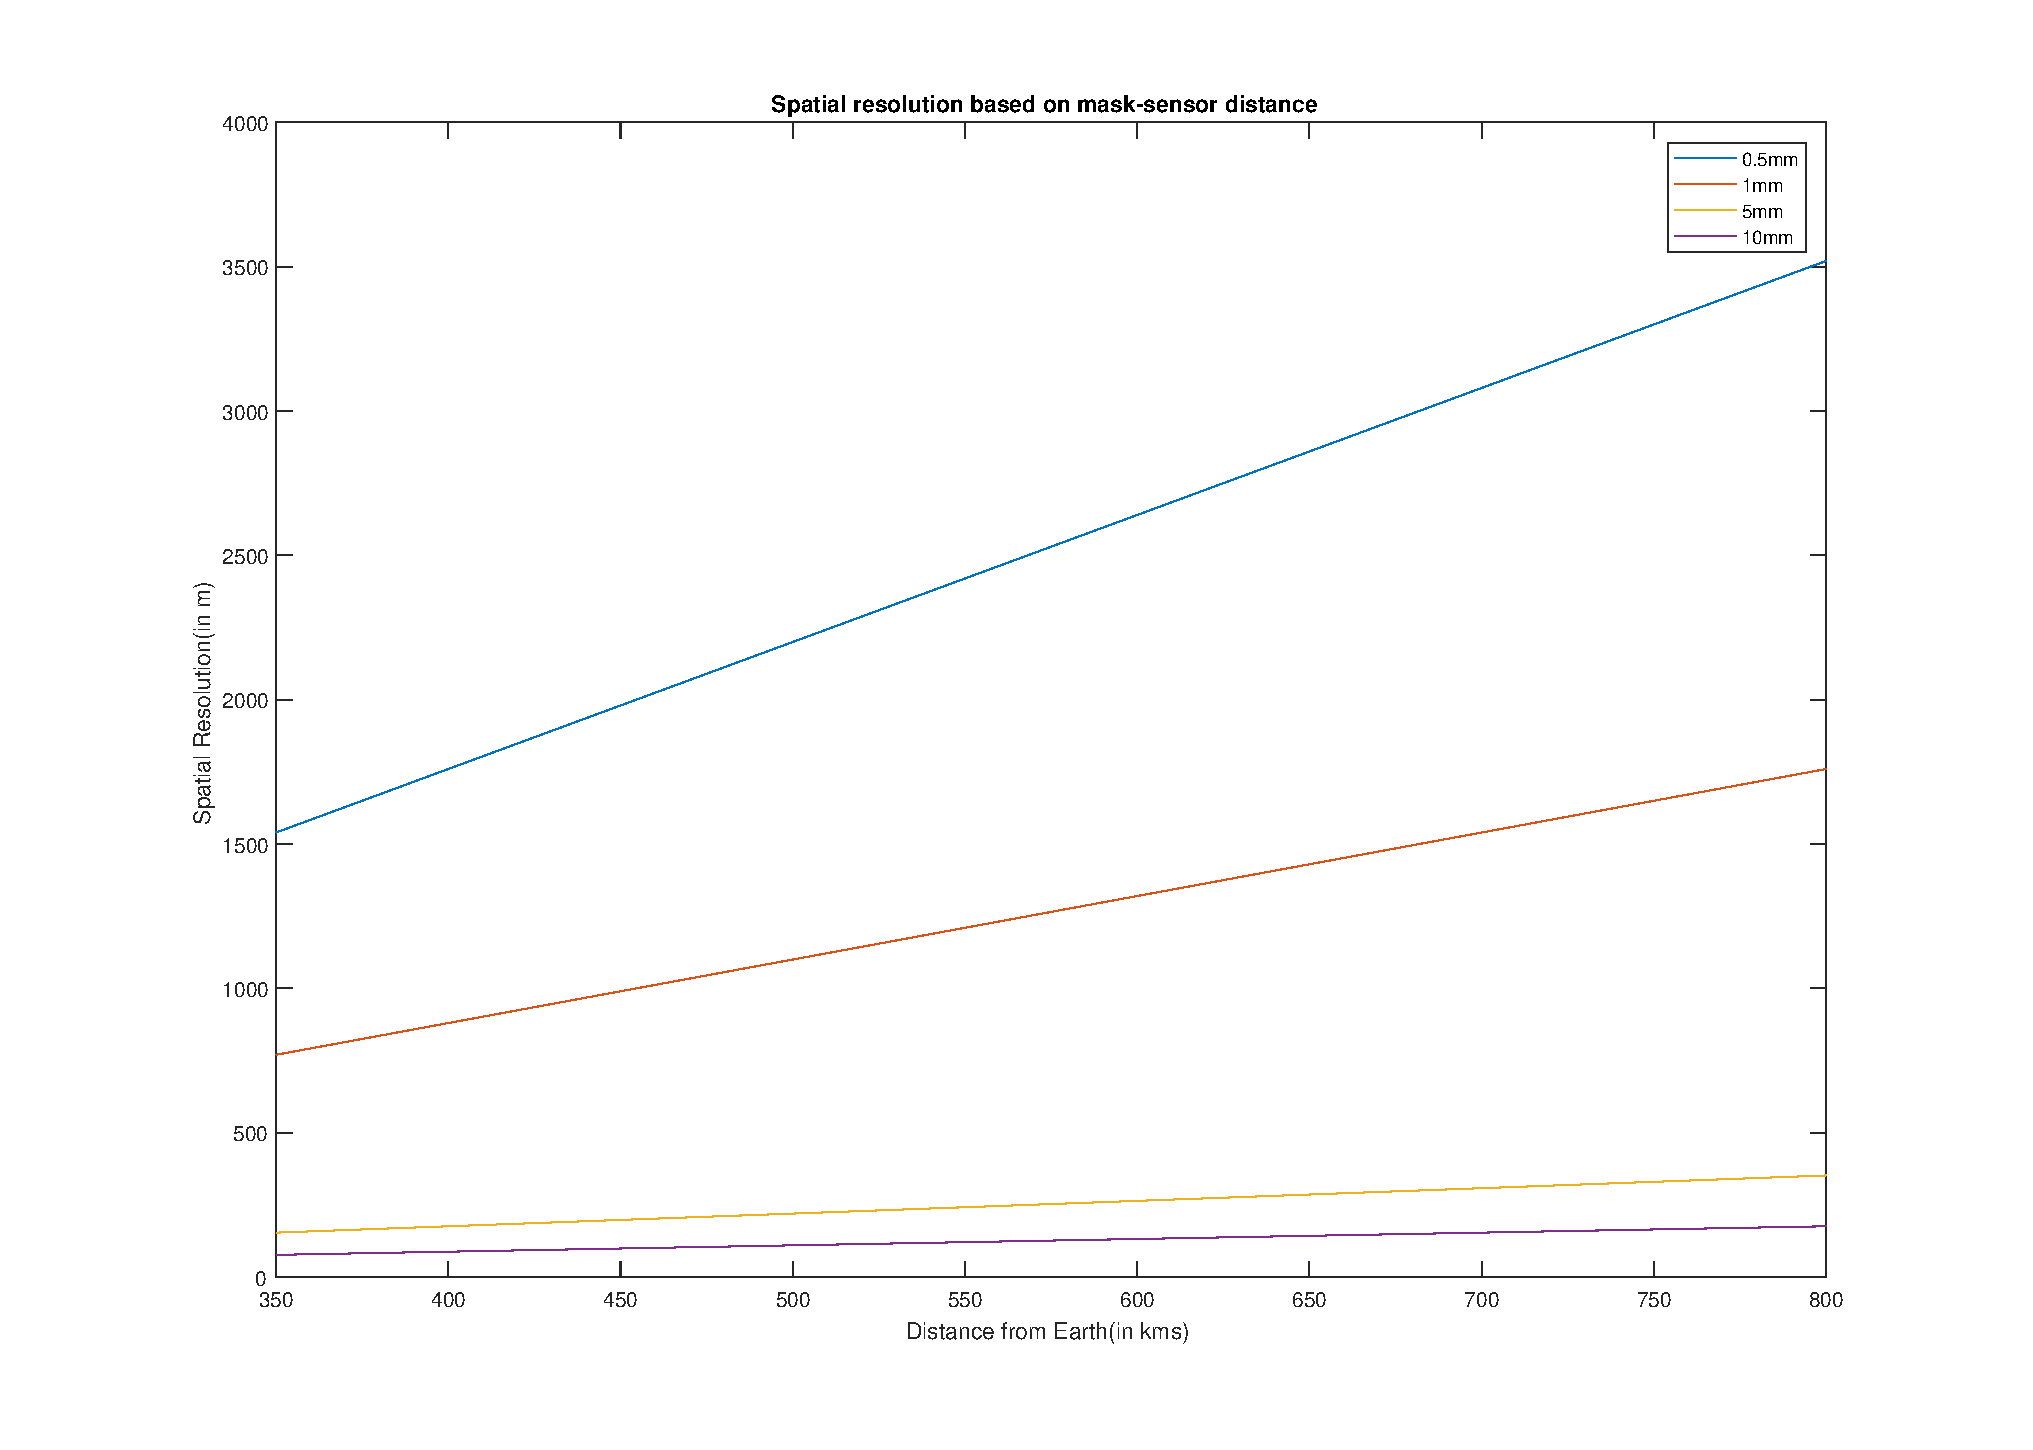
\includegraphics[width = \linewidth]{pics/spatial_res}
\caption{Relation between Spatial resolution and mask-sensor distance for sensor OV2640}
\label{fig:spat-res-graph-1}
\end{figure}

The field of view of the camera can be calculated using the acceptance angle calculated from integrating the experimental and simulation results. The sensor OV2640 has an experimentally verified acceptance angle of 21.7$\degree$($\theta_{cra}$). The field of view can be calculated using equation \ref{eq:fov_calc_2}. 
\begin{equation}
\label{eq:fov_calc_2}
d_{fov} = 2*d_h*tan(\theta_{cra})
\end{equation}
The obtained calculation results are shown in Figure \ref{fig:fov-graph-1}. It can be seen that maximum field of view can be obtained when the satellite is at a height of 800 kilometers from the surface of the earth. However, the spatial resolution as mentioned earlier will be lower at higher altitudes. A maximum field of view of 636 kilometers can be obtained at a height of 800 kilometers. The sensor OV5642 has an acceptance/chief ray angle of 23.6$\degree$ as mentioned in its data sheet\cite{OV5642DS}. However, this claim has not been experimentally verified.

\begin{figure}[]
\centering
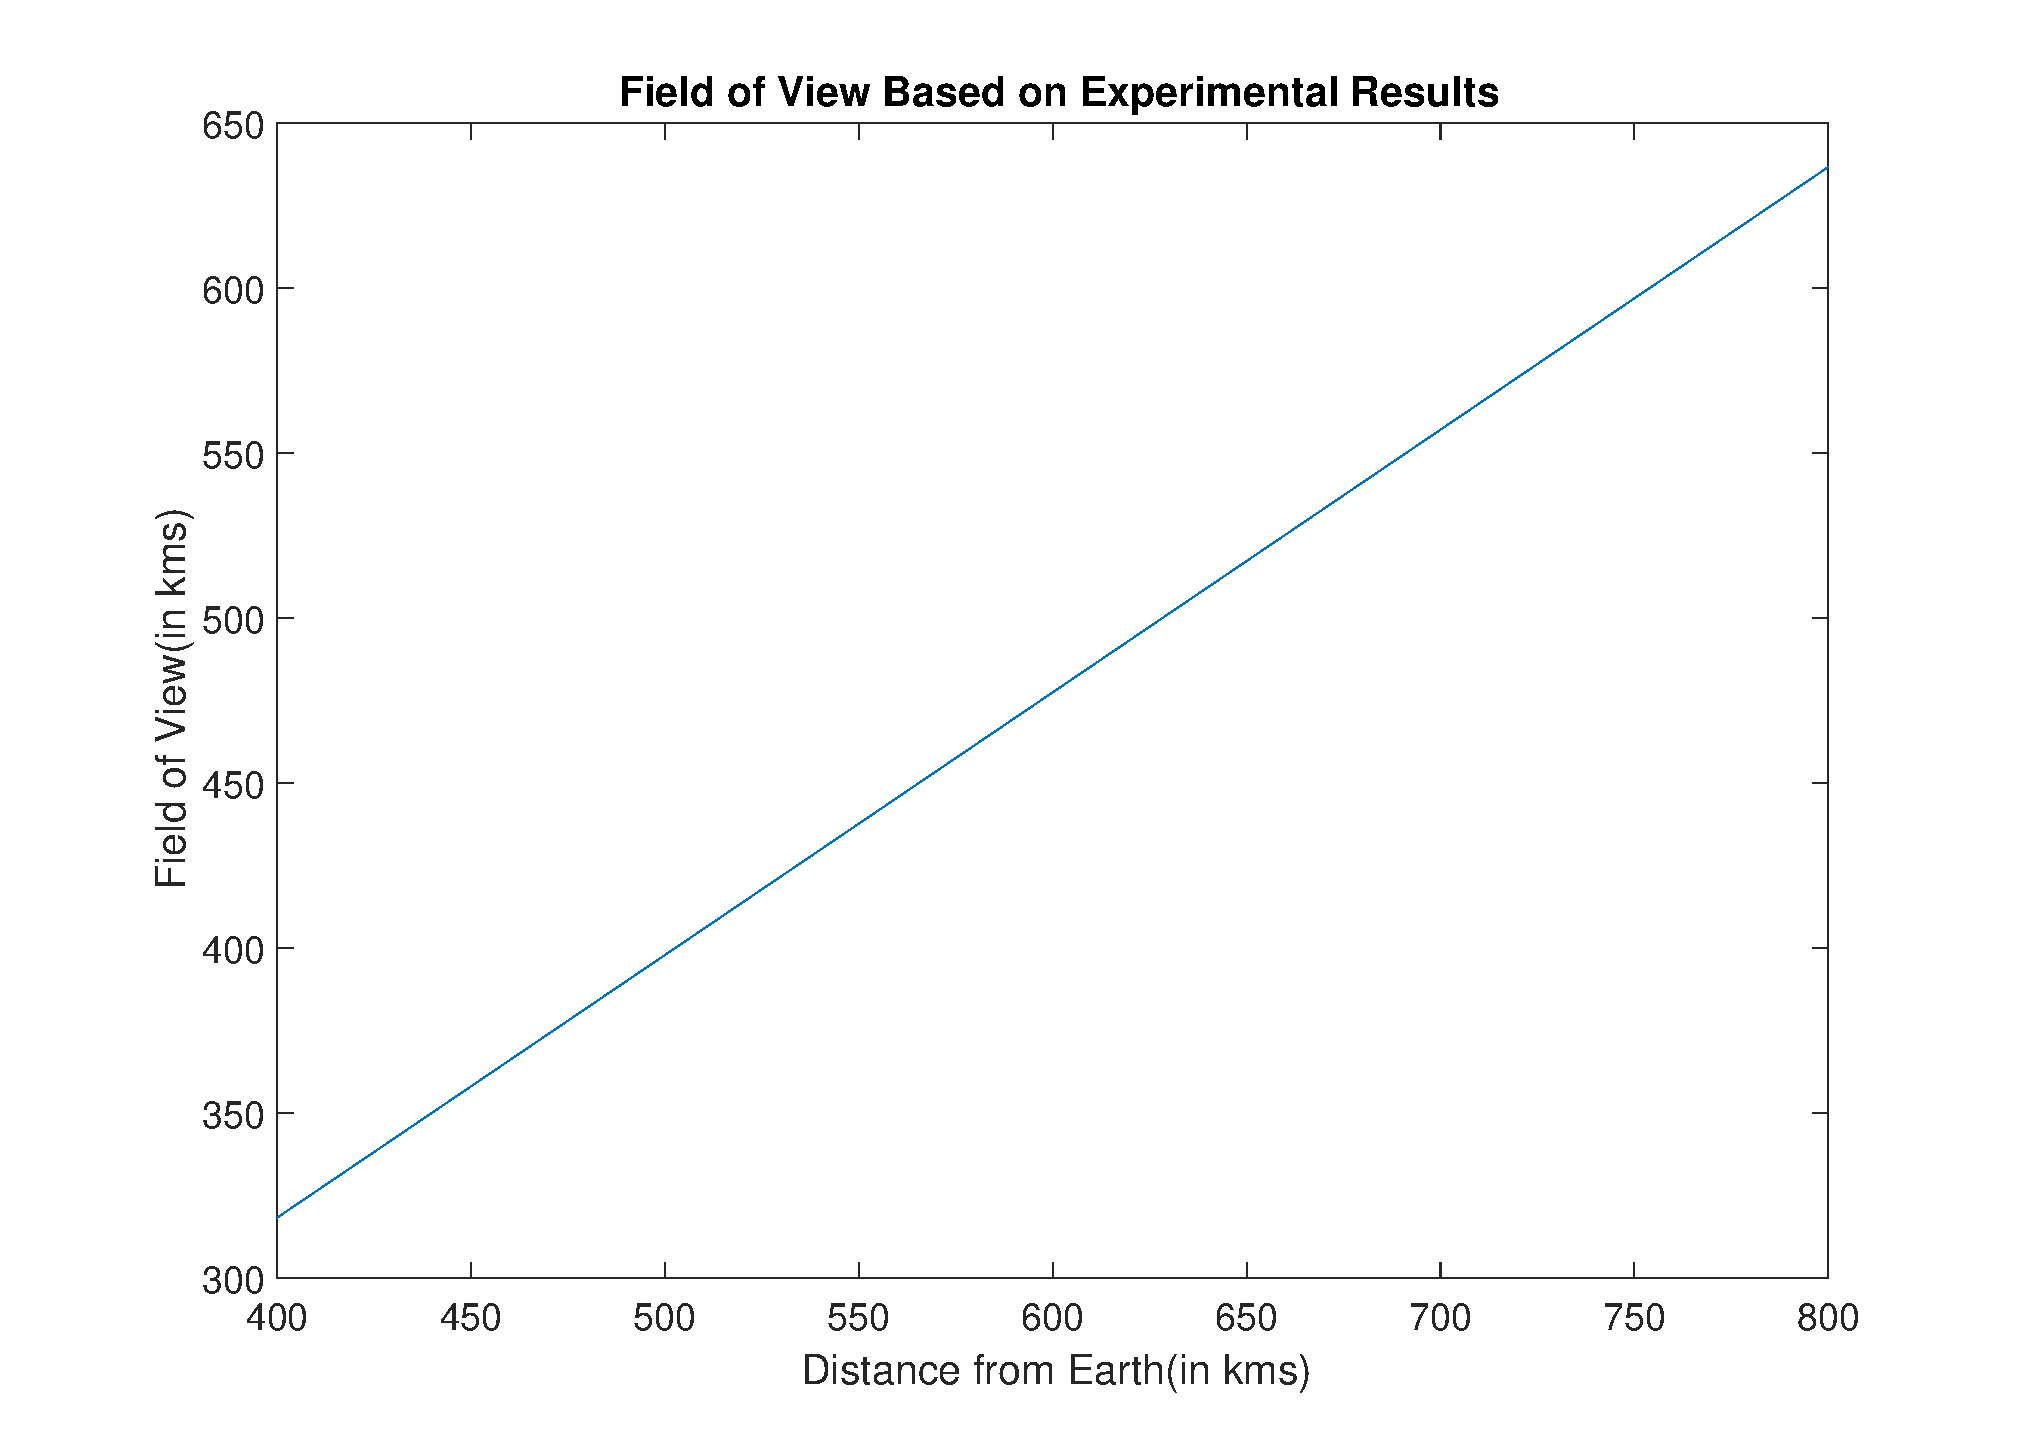
\includegraphics[width = \linewidth]{pics/FOV_Lensless}
\caption{Field of View Calculation based on Experimental Results}
\label{fig:fov-graph-1}
\end{figure}

\section{Spatial Light Modulators}
A spatial light modulator (SLM) is an object that imposes some form of spatially varying modulation on a beam of light\cite{SLMWiki}.SLMs can be controlled by computer controlled software and it would be possible to generate patterns on the SLM that could modulate phase or the intensity of the beam or both simultaneously. An advantage of using an SLM over designing a lithographic mask is that it would be possible to test out different designs of masks quickly in order to find out an optimal mask configuration that would be suitable to our setup. In our design of the lensless imager, it must be possible to block and allow light in a certain binary pattern. A transmissive SLM would suit the purpose of simulating different mask patterns. For this purpose, a Holoeye LC2012 SLM was used. The SLM has a pixel area of $1024 \times 768$ and a pixel pitch of $36\  \mu m$.

\begin{figure}[ht]
\centering
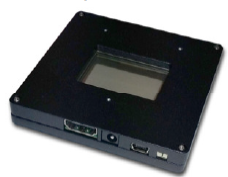
\includegraphics[width=0.50\textwidth]{pics/slm}
\caption{HoloEye LC2012 SLM}
\label{fig:slm}
\end{figure}
